\documentclass[a4paper, 12pt]{article}
% math symbols
\usepackage{amssymb}
\usepackage{amsmath}
\usepackage{mathrsfs}
\usepackage{physsummer}


\usepackage{enumitem}
\usepackage[margin = 2cm]{geometry}

\tolerance = 1000
\emergencystretch = 0.74cm



\pagestyle{empty}
\parindent = 0mm

\begin{document}

\begin{center}
  \Large{\textbf{Городской центр физического образования, 10 класс.}\\
  \textit{Сборы к региону, январские каникулы.}}
\end{center}

\large


\task{ Небольшой груз соскальзывает без начальной скорости по
  наклонной плоскости. Известно, что коэффициент трения между грузом и
  плоскостью меняется по закону $\mu = \alpha x$, где
  $x$~---~расстояние вдоль плоскости от начального положения
  груза. Опустившись на высоту $H$ по вертикали, груз
  останавливается. Найдите максимальную скорость груза в процессе
  движения. }
% Регион-10, 2014

\taskpic{ Идеальный газ в количестве $\nu$ моль участвует в процессе
  $AB$, изображённом на рисунке в координатах $\rho(T)$, где
  $\rho$~---~плотность газа, а $T$~---~его температура. При каких
  условиях (температуре) давление газа на 25\% меньше максимального?
  Температура $T_0$ известна.  }
{
  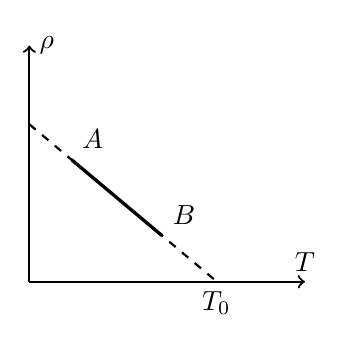
\begin{tikzpicture}
    \draw[thick,->] (0,0) -- (3.5,0) node[above] {$T$};
    \draw[thick,->] (0,0) -- (0,3) node[right] {$\rho$};
    \draw[thick,dashed] (0,2) -- ++(-40:3.1cm) node[below] {$T_0$};
    \draw[very thick] (0,2) ++(-40:0.7cm) node[above right] {$A$} --
    ++(-40:1.5cm) node[above right] {$B$};
  \end{tikzpicture}
}
% Регион-10, 2010

\task{ Четыре резистора сопротивлениями $R_1=3$ Ом, $R_2=4$ Ом,
  $R_3=7$ Ом и $R_4=6$ Ом соединены с батареей, напряжение на которой
  $U_{01}=9{,}1$ В, а её внутренним сопротивлением можно пренебречь.
  \begin{enumerate}
  \item Между резисторами подключен идеальный вольтметр. Найдите его
    показания. В какую сторону отклонится стрелка вольтметра?
    Известно, что при подключении клеммы вольтметра, помеченной
    символом (+), к положительному выводу батареи, а клеммы
    вольтметра, помеченной символом (-), к отрицательному выводу
    батареи, стрелка отклоняется вправо.
  \item Через какое-то время батарея частично разрядилась, и
    напряжение на её выводах уменьшилось до $U_{02}=9{,}0$ В. Вместо
    вольтметра в цепь включили амперметр, сопротивление которого
    пренебрежимо мало. Найдите показания амперметра. В какую сторону
    отклонится его стрелка?
  \end{enumerate}}
\begin{center}
  \begin{tikzpicture}[circuit ee IEC, thick]
    \node[contact] (a) at (0,0) {};
    \node[contact] (b) at (3,0) {};
    \node[contact] (c) at (1.5,1.5) {};
    \node[contact] (d) at (1.5,-1.5) {};
    \draw[thick] (a) to[resistor={info={$R_1$}}] (c)
    to[resistor={info={$R_2$}}] (b) to[resistor={info={$R_4$}}] (d)
    to[resistor={info={$R_3$}}] (a);
    \draw[thick] (c) to[voltmeter] (d);
    \draw (a) ++ (20:1.3cm) node {$+$};
    \draw (a) ++ (-20:1.3cm) node {$-$};
    \draw[thick] (a) -- ++(left:0.5cm) -- ++(down:2cm)
    to[battery={info'={$U_{01}$}}] ++(2,0) to[make contact] ++(2,0) --
    ++(up:2cm) -- (b);  
  \end{tikzpicture}
\end{center}
% Регион-10, 2011


\normalsize

\task{ К двум лёгким подвижным блокам подвешены грузы, массы которых
  $m_1$ и $m_2$. Лёгкая нерастяжимая нить, на которой висит блок с
  грузом $m_1$, образует с горизонтом угол $\alpha$. Грузы удерживают
  в равновесии (см. рис.). Найдите ускорение грузов сразу после того,
  как их освободят. Считайте, что радиусы блоков $r \ll L$.  }
\begin{center}
  \begin{tikzpicture}
    \def\r{0.2cm};
    \draw[interface,thick] (0,0) -- (6,0) -- ++(0,-1.5);
    \coordinate (a) at (0.5cm,-3);
    \coordinate (b) at ({0.5cm+2*\r},-0.5);
    \coordinate (c) at (3.5cm,-1.5);
    \draw[very thick] (a) circle (\r);
    \draw[thick] (a) ++ (-\r,0) |- (0,0);
    \draw[thick] (a) ++ (\r, 0) -- ($(b)+(-\r,0)$); 
    \draw[very thick] (b) circle (\r);
    \draw[thick] (b) -- ++(60:0.57cm);
    \draw[thick] (b) -- ++(120:0.57cm);
    \draw[thick] (b) ++ (45:\r) -- ($(c)+(225:\r)$);
    \draw[thick] (c) ++ (-45:\r) -- (6,-0.37);
    \draw[very thick] (c) circle (\r);
    \draw[blue,thick,<->] (b) ++ (45:\r) --(6,-0.37)
    node[midway,below] {$L$};
    \draw (6,-0.37) ++ (195:1cm) node[blue] {$\alpha$};
    \draw[thick] (a) -- ++(0,-0.5cm);
    \draw[thick] (a) ++ (-0.4cm,-0.5cm) rectangle ++(0.8cm,-0.6cm)
    node[midway] {\small $m_2$};
    \draw[thick] (c) -- ++(0,-0.5cm);
    \draw[thick] (c) ++ (-0.4cm,-0.5cm) rectangle ++(0.8cm,-0.6cm)
    node[midway] {\small $m_1$}; 
  \end{tikzpicture}
\end{center}
% Регион-10, 2014

\task{ Экспериментатор Глюк решил исследовать силу реакции опоры,
  действующую со стороны чаши весов на однородную цепочку. Для этого
  он подвесил цепочку за верхнее звено так, что нижним концом она
  почти касалась чаши электронных весов и затем отпустил её. В момент
  начала падения автоматически запустился электронный
  секундомер. Мгновенные показания весов $P$ и секундомера $t$
  передавались на обработку в компьютер. Результаты измерений
  несколько озадачили экспериментатора:
  \begin{center}
    \begin{tabular}[h]{|l|c|c|c|}
      \hline
      $t$, с & 0,2 & 0,4 & 0,6\\
      \hline
      $P$, грамм & 50 & 200 & 100\\
      \hline
    \end{tabular}
  \end{center}
  По этим данным определите массу $m$ цепочки, её длину $L$ и время
  падения $t_1$. Силами сопротивления воздуха пренебречь, $g=10\mbox{
    м/c}^2$. 
}
% Регион-10, 2013

\taskpic{ В архиве Кельвина нашли рукопись, на которой был изображён
  процесс $1 \to 2 \to 3$, совершённый над одним молем гелия. От
  времени чернила выцвели, и стало невозможно разглядеть, где
  находятся оси давления и объёма. Однако из текста следовало, что
  состояния 1 и 3 лежат на одной изохоре, соответствующей объёму
  $V_{1}$. Кроме того, было сказано, что количество теплоты,
  подведённой в процессе $1 \to 2 \to 3$ к газу, равно
  нулю. Определите объём $V_2$. } {
  \begin{tikzpicture}
    \draw[very thick, marrow] (0,0) node[below] {\textbf{1}} --
    ++(40:3cm) node[right] {\textbf{2}};
    \draw[very thick, marrow] (0,0) ++ (40:3cm) -- (0,1.2) node[above]
    {\textbf{3}}; 
  \end{tikzpicture}
}
% Регион-10, 2011

\taskpic[3cm]{ Металлический куб прикреплён в точке \textbf{A} к тяжёлой
  однородной верёвке, перекинутой через два лёгких блока. Другой конце
  верёвки закреплён на неподвижной опоре в точке \textbf{B} так, то
  точки \textbf{A} и \textbf{B} находятся на одинаковой высоте. Силы
  $F_1=110$ Н и $F_2=90$ Н, приложенные к осям блоков, удерживают
  систему в равновесии. Определите длину верёвки $L$. Линейная
  плотность верёвки (масса единицы длины) равна
  $\rho=0{,}25 \mbox{ кг/м}$, а $g=10 \mbox{ м/с}^2$. Трения в осях
  блоков нет. Радиусом блоков по сравнению с длиной верёвки
  пренебречь нельзя. }
{
  \begin{tikzpicture}
    \def\r{0.25cm};
    \coordinate (a) at (1.5,1.5); 
    \coordinate (b) at (2,-1.5); 
    \draw[thick,interface] (2,0) -- (3,0);
    \draw[thick] (2,0) ++ (right:\r) node[above] {\textbf{B}} --
    ++(down:1.5cm); 
    \draw[very thick] (b) circle (\r);
    \draw[thick] (2,-1.5) ++ (left:\r) -- ++(up:3cm);
    \draw[very thick] (a) circle (\r);
    \draw[thick] (a) ++ (left:\r) -- ++(down:1.5cm) node[above left]
    {\textbf{A}}; 
    \draw[thick] (a) ++ (-2*\r,-1.5cm) rectangle ++(2*\r,-0.5cm);
    \draw[thick,->] (a) -- ++(up:1cm) node[right] {$\vec{F}_1$};
    \draw[thick,->] (b) -- ++(down:1cm) node[right] {$\vec{F}_2$}; 
  \end{tikzpicture}
}
% Регион-10, 2011

\taskpic[5.5cm]{ Диаметр входного отверстия воздухопровода тепловой пушки
  $D_1=20$ см, выходного --- $D_2=22$ см. При стационарной работе
  вентилятора и нагревателя скорость воздуха $v=1{,}5$ м/с на входе и
  выходе оказалась одинаковой при разных давлениях $p_1=10^5$ Па и
  $p_2=1{,}05 \cdot 10^5$ Па. Найдите температуру $t_2$ воздуха на
  выходе и мощность $N$, потребляемую тепловой пушкой. Температура
  воздуха на входе в пушку равна $t_1=7^{\circ}$C.   }
{
  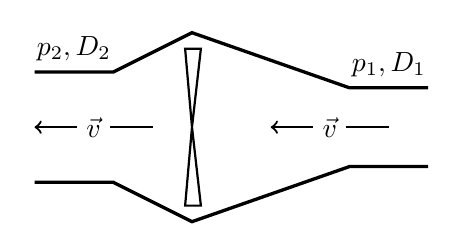
\begin{tikzpicture}
    \draw[very thick] (0,0.2) -- (1,0.2) node[midway,above] {$p_2, D_2$}
    -- (2,0.7) -- (4,0) -- (5,0) node[midway,above] {$p_1, D_1$}; 
    \draw[very thick] (0,-1.2) -- (1,-1.2) -- (2,-1.7) -- (4,-1) -- (5,-1);
    \draw[thick] (2,-0.5) -- ++(95:1cm) -- ++(right:0.2cm) -- (2,-0.5)
    -- ++(265:1cm) -- ++(right:0.2cm) -- (2,-0.5);
    \draw[thick,->] (1.5,-0.5) -- ++(left:1.5cm)
    node[midway,fill=white] {$\vec{v}$};
    \draw[thick,->] (4.5,-0.5) -- ++(left:1.5cm)
    node[midway,fill=white] {$\vec{v}$};  
  \end{tikzpicture}
}
% Регион-10, 2013

\task{ Теоретик Баг предложил экспериментатору Глюку определить схему
  электрического чёрного ящика (ЧЯ) с двумя выводами. В ящике
  находятся два одинаковых диода и два разных резистора. Вольтамперная
  характеристика (ВАХ) чёрного ящика приведена на левом рисунке, а ВАХ
  диода --- на правом. Восстановите схему ЧЯ и определите
  сопротивление каждого из резисторов. }
\begin{figure}[h]
  \centering
  \subcaptionbox{ВАХ чёрного ящика.}
    {\begin{tikzpicture}
      \draw[thick,->] (-0.1,0) -- (4,0) node[above] {$U$, В};
      \draw[thick,->] (0,-0.1) -- (0,3.5) node[left] {$I$, мА};
      \foreach \x in {0.5,1,...,3.5} {\draw[thick] (\x,0.1) --
        ++(0,-0.2);}
      \foreach \y in {0.3,0.6,...,3.4} {\draw[thick] (0.1,\y) --
        ++(-0.2,0);}
      \draw[very thick] (1,0) -- (2.5,1.5) -- (3,3);
      \draw[dashed,thick] (3,3) |- (0,0);
      \draw[dashed,thick] (3,3) -| (0,0);
      \draw[dashed,thick] (2.5,1.5) |- (0,0);
      \draw[dashed,thick] (2.5,1.5) -| (0,0);
      \draw (1,0) node[below] {0,5};
      \draw (2,0) node[below] {1,0}; 
      \draw (3,0) node[below] {1,5};
      \draw (0,0.6) node[left] {10};
      \draw (0,1.2) node[left] {20};
      \draw (0,1.8) node[left] {30}; 
      \draw (0,2.4) node[left] {40}; 
    \end{tikzpicture}}
    \qquad
    \subcaptionbox{ВАХ диода.}
    {\begin{tikzpicture}
      \draw[thick,->] (-0.1,0) -- (4,0) node[above] {$U$, В};
      \draw[thick,->] (0,-0.1) -- (0,3.5) node[left] {$I$};
      \draw[thick] (1.5,0.1) -- ++(0,-0.2) node[below] {0,5};
      \draw[thick] (3,0.1) -- ++(0,-0.2) node[below] {1,0};
      \draw[very thick] (1.5,0) -- ++(0,3.5); 
    \end{tikzpicture}}
\end{figure}
% Регион-10, 2014

\task{ Электрическая цепь состоит из батарейки, шести резисторов,
  значения сопротивлений которых $R_1=1$ кОм, $R_2=2$ кОм, $R_3=3$
  кОм, $R_4=4$ кОм и трёх одинаковых амперметров, внутреннее
  сопротивление $r$ которых мало ($r \ll R_1$). Вычислите показания
  амперметров, если напряжение батарейки $U=3{,}3$ В.  }
\begin{figure}[h]
  \centering
  \begin{tikzpicture}[circuit ee IEC,thick]
    \node[contact] (12) at (2,2) {}; 
    \node[contact] (13) at (4,2) {};
    \node[contact] (21) at (0,0) {};
    \node[contact] (22) at (2,0) {}; 
    \node[contact] (23) at (4,0) {}; 
    \node[contact] (32) at (2,-2) {}; 
    \node[contact] (33) at (4,-2) {};

    \draw[thick] (21) -- (22) node[midway,circle,draw,fill=white]
    {$A_2$};  
    \draw[thick] (22) -- (23) node[midway,circle,draw,fill=white]
    {$A_1$};  
    \draw[thick] (21) to[resistor={info={$R_3$}}] ++(0,2) -- (12)
    to[resistor={info={$R_3$}}] (22) 
    to[resistor={info={$R_2$}}] (32) -- ++(-2,0)
    to[resistor={info={$R_1$}}] (21); 
    \draw[thick] (12) -- (13) to[resistor={info={$R_3$}}] (23)
    to[resistor={info={$R_4$}}] (33) -- (32); 
    \draw[thick] (21) -- ++(-1,0) -- ++(0,3) -- ++(6,0)
    node[midway,circle,draw,fill=white] {$A_3$} -- ++(0,-3) --
    (23);
    \draw[draw=white,double=black,double distance=\pgflinewidth,ultra
    thick] (13) -- ++(2,0) to[battery={info={$U$}}] ++(0,-4) -- (33); 
  \end{tikzpicture}
\end{figure}
% Регион-10, 2013

\end{document}


%%% Local Variables: 
%%% mode: latex
%%% TeX-engine:xetex
%%% TeX-PDF-mode: t
%%% End:
